%%%%%%%%%%%%%%%%%%%%%%%%%%%%%%%%%%%%%%%%%
% a0poster Landscape Poster
% LaTeX Template
% Version 1.0 (22/06/13)
%
% The a0poster class was created by:
% Gerlinde Kettl and Matthias Weiser (tex@kettl.de)
% 
% This template has been downloaded from:
% http://www.LaTeXTemplates.com
%
% License:
% CC BY-NC-SA 3.0 (http://creativecommons.org/licenses/by-nc-sa/3.0/)
%
%%%%%%%%%%%%%%%%%%%%%%%%%%%%%%%%%%%%%%%%%

%----------------------------------------------------------------------------------------
%	PACKAGES AND OTHER DOCUMENT CONFIGURATIONS
%----------------------------------------------------------------------------------------

\documentclass[a0,landscape]{a0poster}

\usepackage{multicol} % This is so we can have multiple columns of text side-by-side
\columnsep=50pt % This is the amount of white space between the columns in the poster
\columnseprule=3pt % This is the thickness of the black line between the columns in the poster

\usepackage[svgnames]{xcolor} % Specify colors by their 'svgnames', for a full list of all colors available see here: http://www.latextemplates.com/svgnames-colors

\usepackage{times} % Use the times font
%\usepackage{palatino} % Uncomment to use the Palatino font

\usepackage{graphicx} % Required for including images
\graphicspath{{figures/}} % Location of the graphics files
\usepackage{booktabs} % Top and bottom rules for table
\usepackage[font=small,labelfont=bf]{caption} % Required for specifying captions to tables and figures
\usepackage{amsfonts, amsmath, amsthm, amssymb} % For math fonts, symbols and environments
\usepackage{wrapfig} % Allows wrapping text around tables and figures
\usepackage[document]{ragged2e}
\usepackage{enumitem}
\usepackage{graphicx}
%\usepackage[usenames,dvipsnames]{color}
\usepackage{hyperref}

\begin{document}
\noindent
%----------------------------------------------------------------------------------------
%	POSTER HEADER 
%----------------------------------------------------------------------------------------

% The header is divided into three boxes:
% The first is 55% wide and houses the title, subtitle, names and university/organization
% The second is 25% wide and houses contact information
% The third is 19% wide and houses a logo for your university/organization or a photo of you
% The widths of these boxes can be easily edited to accommodate your content as you see fit

\begin{minipage}[b]{0.55\linewidth}
\veryHuge \color{NavyBlue} \textbf{NoSQL Data Mangement Systems} \color{Black}\\ % Title
\Huge\textit{A Very Subtle Introduction}\\[1cm] % Subtitle
\huge \textbf{Hassan Abedi}\\ % Author(s)
\huge School of Computer Engineering - IUST\\ % University/organization
\end{minipage}
%
\begin{minipage}[b]{0.25\linewidth}
\color{DarkSlateGray}\Large \textbf{How to reach me:}\\
%School of Computer Engineering\\ % Address
%Iran University of Science and Technology\\
%123 Broadway, State, Country\\\\
%Phone: +1 (000) 111 1111\\ % Phone number
Email: \texttt{hassan.abedi.t@gmail.com}\\ % Email address
\end{minipage}
%
\begin{minipage}[b]{0.19\linewidth}
\includegraphics[width=20cm]{logo.jpg} % Logo or a photo of you, adjust its dimensions here
\end{minipage}

\vspace{1cm} % A bit of extra whitespace between the header and poster content

%----------------------------------------------------------------------------------------

\begin{multicols}{4} % This is how many columns your poster will be broken into, a poster with many figures may benefit from less columns whereas a text-heavy poster benefits from more

\color{DarkSlateGray} 
\section*{What NoSQL is and what it is not}
\justifying {

NoSQL really is a generic term about data storage systems used in storing and retriving the type of data which isn't in the classical tabular form, like as it's a Realational Database. Actually  some may claim is NoSQL not even about a type of database but more of a something that is not SQL.
NoSQL trys to answer to three main needs in short:
}\par

\color{DarkSlateBlue} 
\begin{list}{$\circ$}{}

\renewcommand{\labelitemi}{$\bullet$}

\item \justifying  {
They provide \textbf{horizontal scaling}.
 }\par
\item \justifying  {
They provide really high levels of \textbf{availability}.
 }\par
\item \justifying  {
They manage to \textbf{store and handle more data types}(like key-values or graph) than RDBMS, so they maybe \textbf{more flexible}.
 }\par

 \end{list}

 \color{DarkSlateGray} 
 \noindent
\justifying 

{
%Because of the need to provide curated information from large volumes, generally in near
% real-time, NoSQL mostly follows a horizontal structure. In geneal they are optimized for
% insert and retrieve operations on a large scale with built-in capabilities for replication
% and clustering. Some of the functionalities of SQL databases like functions, stored
% procedures may not be present in most of the databases.\\
It's not bad to note, for ends mentioned above to manifest most NoSQL stores lack true ACID instead they manage to provide three main features[1]:
\color{DarkSlateBlue} 
\begin{list}{$\circ$}{}

\renewcommand{\labelitemi}{$\bullet$}

\item \justifying  {
\textbf{Basic availability}: Each request is guaranteed a response—successful or
failed execution.
 }\par
\item \justifying  {
 \textbf{Soft state}: The state of the system may change over time, at times without
any input (for eventual consistency).

 }\par
\item \justifying  {
 \textbf{Eventual consistency}: The database may be momentarily inconsistent but
will be consistent eventually.

 }\par
 \end{list}
 
 \color{DarkSlateGray} 
Maybe the biggest difference they make is about data consistency, where most of NoSQL family loosend usual consistency promises a normal RDBMS holds to some sort of In-Future(Eventual) plans to make data consistent.In the moment they are finding significant and growing industry use in  \textbf{Big Data and real-time web applications}. Some people may interpret NoSQL as ``Not Only SQL'' (more serious proponents of them would tell you it stands for ``No to SQL''!;0) reminding that they may deployed besides a RDBMS or atleast may have SQL like query languages like their older cousins.
Data replication is a classical way to get high availability, it's one of main features of NoSQLs, so always remember when someone says i store my data using a NoSQL database she means there is at-least one replica of her data stored somewhere!.\\
Most of NoSQLs compromise consistency (in the sense of the CAP theorem) in favour of availability and partition tolerance.}
\par

\begin{center}\vspace{1cm}
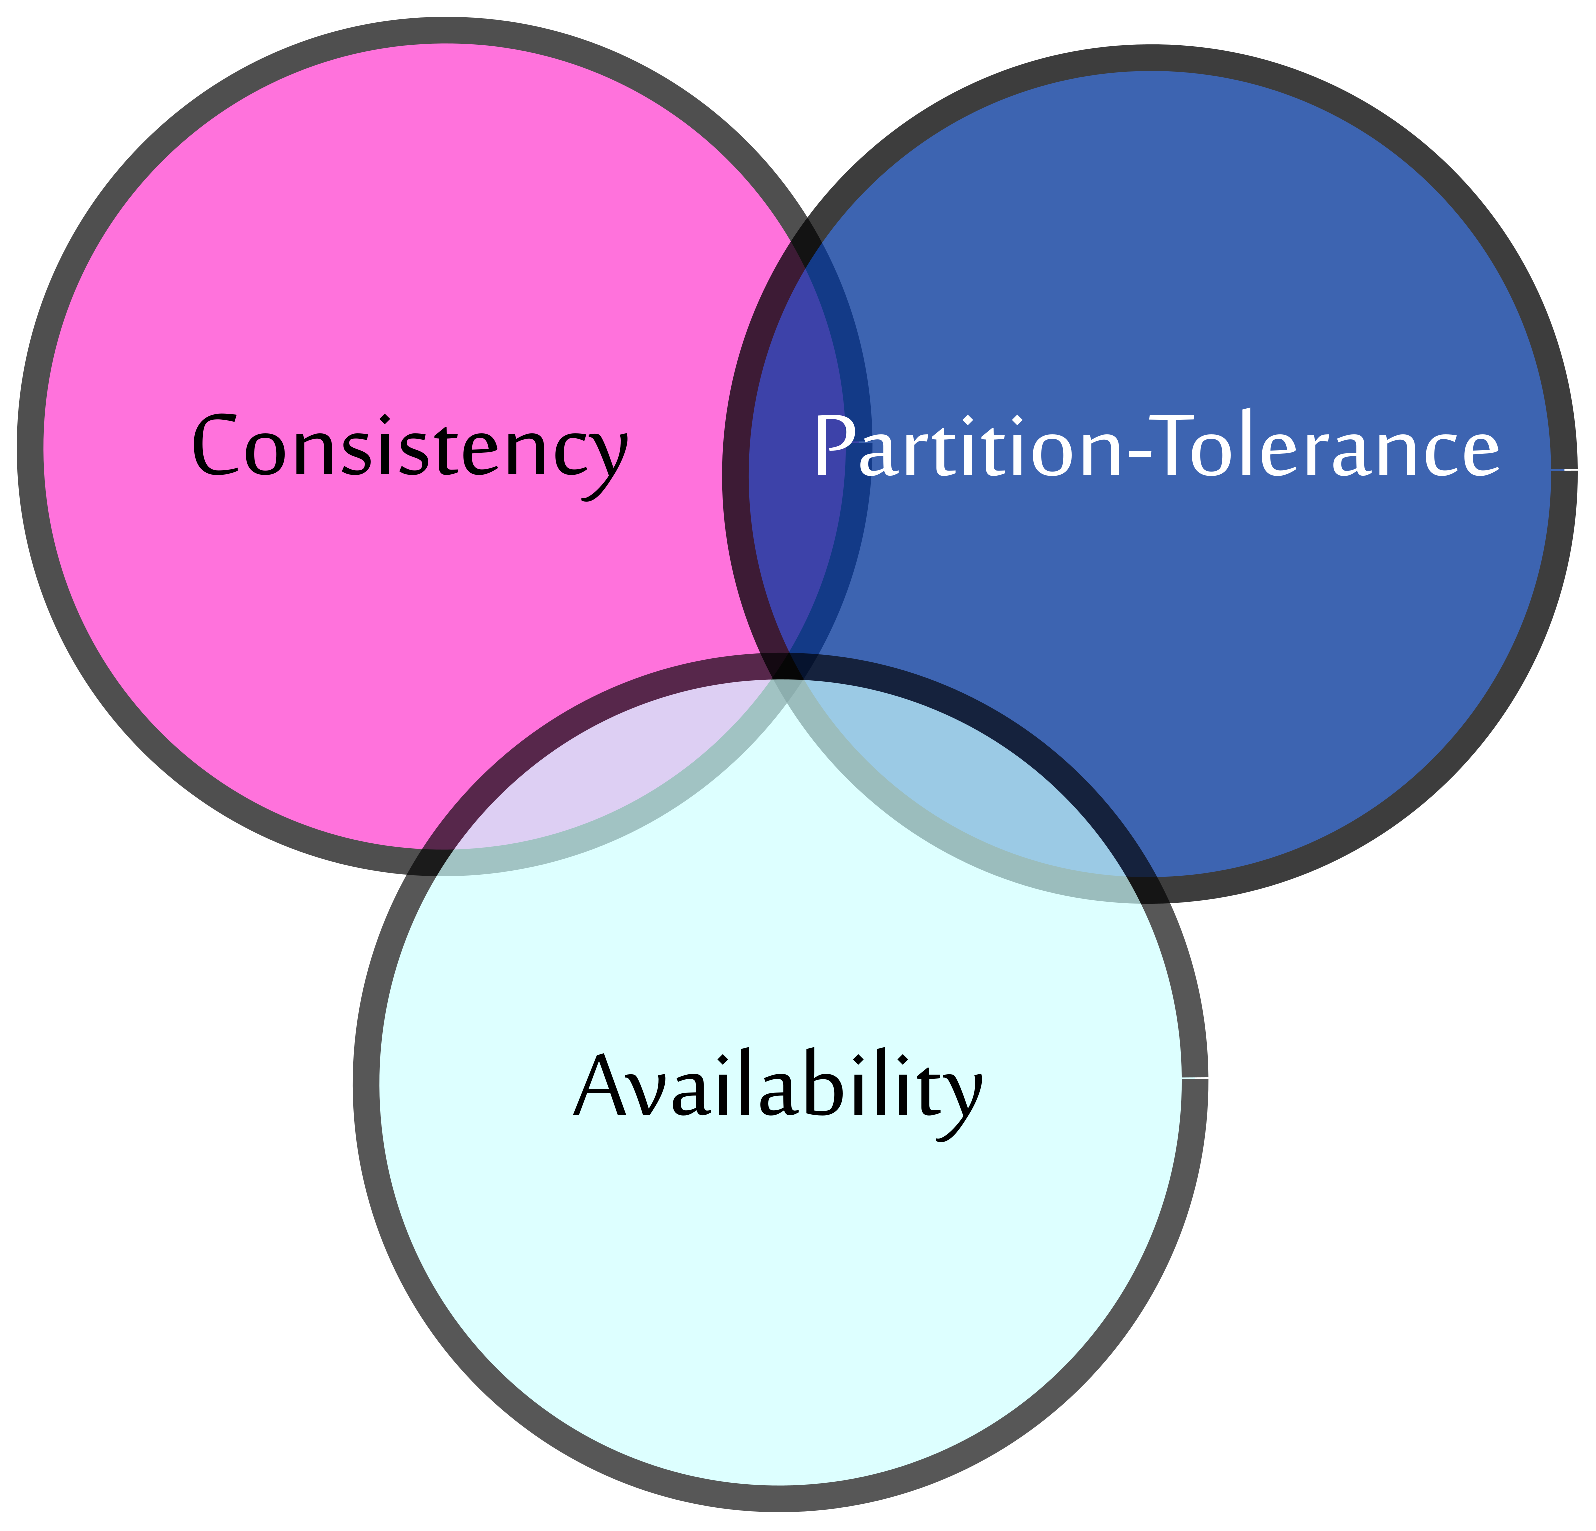
\includegraphics[width=0.60\linewidth]{cap.eps}
\captionof{figure}{\color{Green} Brewer's CAP theorem states you can only have two out of three of C.A.P. at a moment in a distributed computing system.}
\end{center}\vspace{1cm}


%----------------------------------------------------------------------------------------
%	OBJECTIVES
%----------------------------------------------------------------------------------------

\color{DarkSlateGray} % DarkSlateGray color for the rest of the content

\section*{Types of NoSQLs}
\justifying {
\indent
% Because of the need to provide curated information from large volumes, generally in near
% real-time, NoSQL mostly follows a horizontal structure. In geneal they are optimized for
% insert and retrieve operations on a large scale with built-in capabilities for replication
% and clustering. Some of the functionalities of SQL databases like functions, stored
% procedures may not be present in most of the databases.\\
%Also
NoSQL storage management systems usually depending the data that they are designed to store are categorized into different types enumerated below:

}\par

% \color{DarkSlateBlue} 
% \begin{list}{$\circ$}{}
% 
% %\itemsep1em
% 
% \renewcommand{\labelitemi}{$\bullet$}
% 
% \item \justifying  {
% \textbf{Column-oriented stores}.
%  }\par
% \item \justifying  {
% \textbf{Document stores}.
%  }\par
% \item \justifying  {
%  \textbf{Key Value stores}
%  }\par
%  \item \justifying  {
%  \textbf{Graph}
%  }\par
% 
% 
%  \end{list}
 \color{DarkSlateGray} 
\subsection*{Column-oriented stores}

\justifying 
{The column-oriented databases store data as columns as opposed to rows that
is prominent in RDBMS, you can add columns and don't worry about default values for cells in added rows. For these databases there are advantages when working with a subset of the available columns. For example, computing maxima, minima, averages and sums, specifically on large
datasets, is where these column-oriented data stores outshine in performance.
Similarly, when new values are applied for either all rows at once or with same 
column filters, these databases will allow partial data access without touching
unrelated columns and be much faster in execution.\\
Examples:Apache Cassandra, Hbase, Google BigTable
}

\begin{center}\vspace{1cm}
\includegraphics[width=0.8\linewidth]{nosqlx}
\captionof{figure}{\color{Green} NoSQL use is growing every day}
\end{center}\vspace{1cm}


\subsection*{Document stores}
\justifying{
Also referred to as document-oriented database, a document store allows the
inserting, retrieving, and manipulating of semi-structured data. Most of the
databases available under this category use XML, JSON, BSON, or YAML, with
data access typically over HTTP protocol using RESTful API or over Apache Thrift
protocol for cross-language interoperability.
compared to RDBMS, the documents themselves act as records (or rows), however,
it is semi-structured as compared to rigid RDBMS. they provide dynamic or changeable schema or even schema-less documents. because of the limitless flexibility provided in this model, this is one of the more popular models implemented and used.\\
Examples : MongoDB, CouchDB, Terrastore, BaseX
}\par




\subsection*{Key-value stores}
\justifying{
A Key-value store is very closely related to idea of a map in computer science, they are actually distributed hash-tables that store data blobs in arbitrary sizes with unique keys over some distributed buckets. the key part of data usually can be chosen to be of type of string or numerical value but the value section of data - as said earlier - can be almost anything and is allowed to be very large in size.
these databases reach very high performances and are very simpler to design and develop compared to others of their kin. they are optimized for querying against keys, As such they serve great in-memory caches. data usually is accessed via RESTful API(like in Document stores) and only the CRUD operations are supported by the system per-se most of the time.\\
Examples : Redis, Voldemort , Riak, MemcacheDB
}\par

%----------------------------------------------------------------------------------------
%	MATERIALS AND METHODS
%----------------------------------------------------------------------------------------

\subsection*{Graph stores}
\justifying{
Graph databases represent a special category of NoSQL databases where
relationships are represented as graphs. the relationships represented may include social relationships between people, transport links between places, or network topologies between connected systems. they can be considered as special purpose NoSQL databases optimized for relation-heavy data. If there is no relationship among the entities, there is no use-case for graph databases. graph databases are the \textbf{most complex} type of NoSQL databases to build. there is no standard query language yet but graph traversal languages like \textbf{Gremlin} could be used to describe operations over stored graphs.\\
Examples : FlockDB, Neo4j, Titan
}\par

\begin{center}\vspace{1cm}
\begin{tabular}{l l l l l l}
\toprule
\textbf{Features} & \textbf{Column} & \textbf{Document} & \textbf{Key-Value} & \textbf{Graph} \\
\midrule
Table-like schema & yes & no & no & yes \\
Complete update & yes & yes & yes & yes \\
Partial update & yes & yes & yes & no \\

Aggregates across rows & yes & no & no & no \\
Relationships among entities & no & no & no & yes \\
Cross-entity view support & no & yes & no & no \\

Query & yes & yes & no & yes \\
Batch data update & yes & yes & yes & no \\
Batch data fetch & yes & yes & yes & yes \\

\bottomrule
\end{tabular}
\captionof{table}{\color{Green} NoSQL common feaures comparison}
\end{center}\vspace{1cm}

%----------------------------------------------------------------------------------------
\subsection* {Multi-type storages}
\justifying{
There are some intriguing and exceptional example databases that can be categorized differently, mostly they can support multiple data storage plans.
some examples are:
\color{DarkSlateBlue} 
\begin{list}{$\circ$}{}

%\itemsep1em

\renewcommand{\labelitemi}{$\bullet$}

\item \justifying  {
\textbf{OrientDB}{: Supports document storage, key-value as well as graph. \\The official
website is \hyperlink{http://www.orientdb.org}{http://www.orientdb.org}.}
 }\par
\item \justifying  {
\textbf{ArangoDB}{: Universal database with support for document store, key-value
and graph models.\\Official website is \hyperlink{http://www.arangodb.org}{http://www.arangodb.org}.}
 }\par
\item \justifying  {
 \textbf{Aerospike}{: A hybrid between RDBMS
and NoSQL store. it supports document store, key-value, graph as well as
RDBMS. \\Source code can be found at \hyperlink{https://github.com/JakSprats/Alchemy-Database}{https://github.com/JakSprats/Alchemy-Database}.
}
 }\par

 \end{list}

}\par

%\subsection* {Comparisons}



\begin{center}\vspace{1cm}
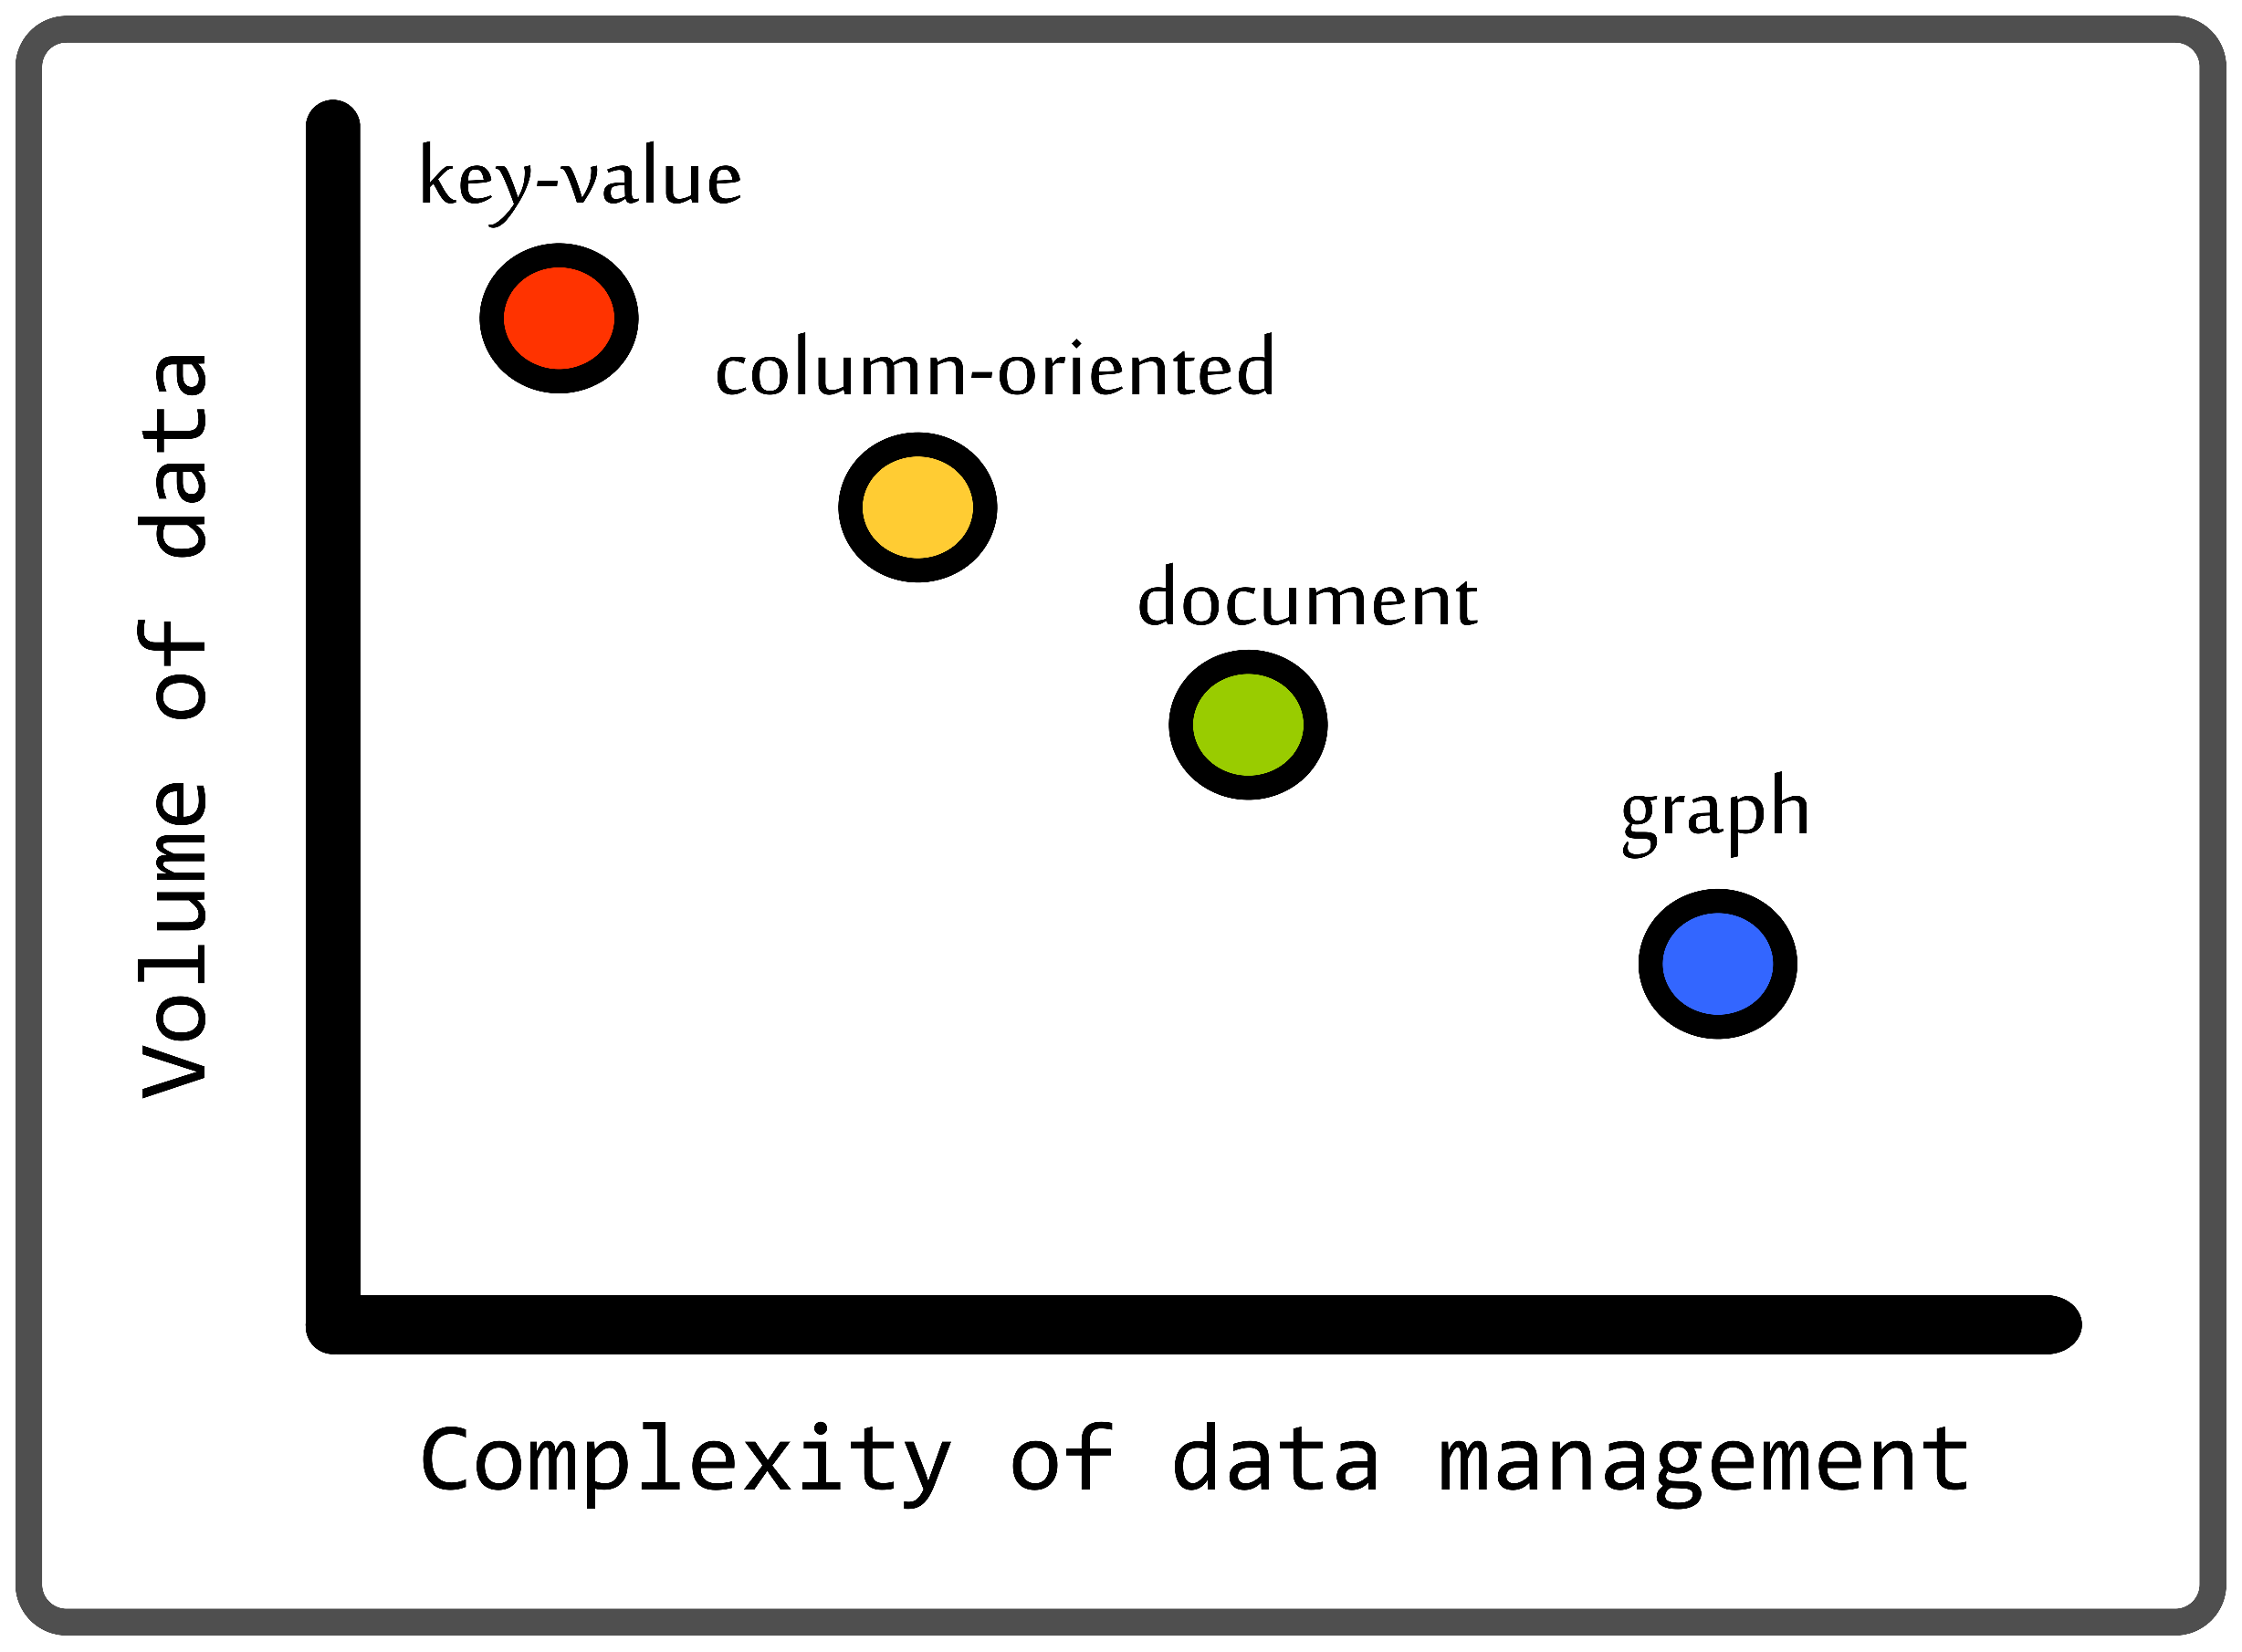
\includegraphics[width=0.8\linewidth]{nosl-complexity}
\captionof{figure}{\color{Green} Data size vs Data complexity in NoSQL family}
\end{center}\vspace{1cm}

\color{DarkRed}
% \subsection*{Criticism of NoSQLs}
% \justifying  {
% A recent critical paper[1] by C.Mohan argues that “while simplicity was touted by some as the reason for going with NoSQL compared to relational as the data model with SQL as the query language, in fact some of the NoSQL systems’ data models are pretty complicated. unlike in the case RDBMSs, for which a whole range of database design tools have been developed over the decades to make the database administrator’s job easier for making design choices there are no such tools available for the NoSQL systems with complex data models.” in another word we better find ways to improve our data management systems with relational model in mind witch has an abundance of tools and methodologies instead of completely trusting NoSQL phenomenon which maybe susceptible to what had been solved for relational databases decades ago.
% }\par
% \color{DarkSlateGray} % Set the color back to DarkSlateGray for the rest of the content

%----------------------------------------------------------------------------------------
%	REFERENCES
%----------------------------------------------------------------------------------------
\nocite{*} % Print all references regardless of whether they were cited in the poster or not
\bibliographystyle{plain} % Plain referencing style
\bibliography{references} % Use the example bibliography file sample.bib

\end{multicols}
\end{document}